%% ----------------------------------------------------------------
%% AppendixA.tex Circuit Diagrams
%% ---------------------------------------------------------------- 
\chapter{Circuit Diagrams} \label{Chapter:AppendixA:CircuitDiagrams}
\section{OV7670 Breakout Board Schematic}\label{sch:OV7670}
\begin{figure}[ht!]
\centering
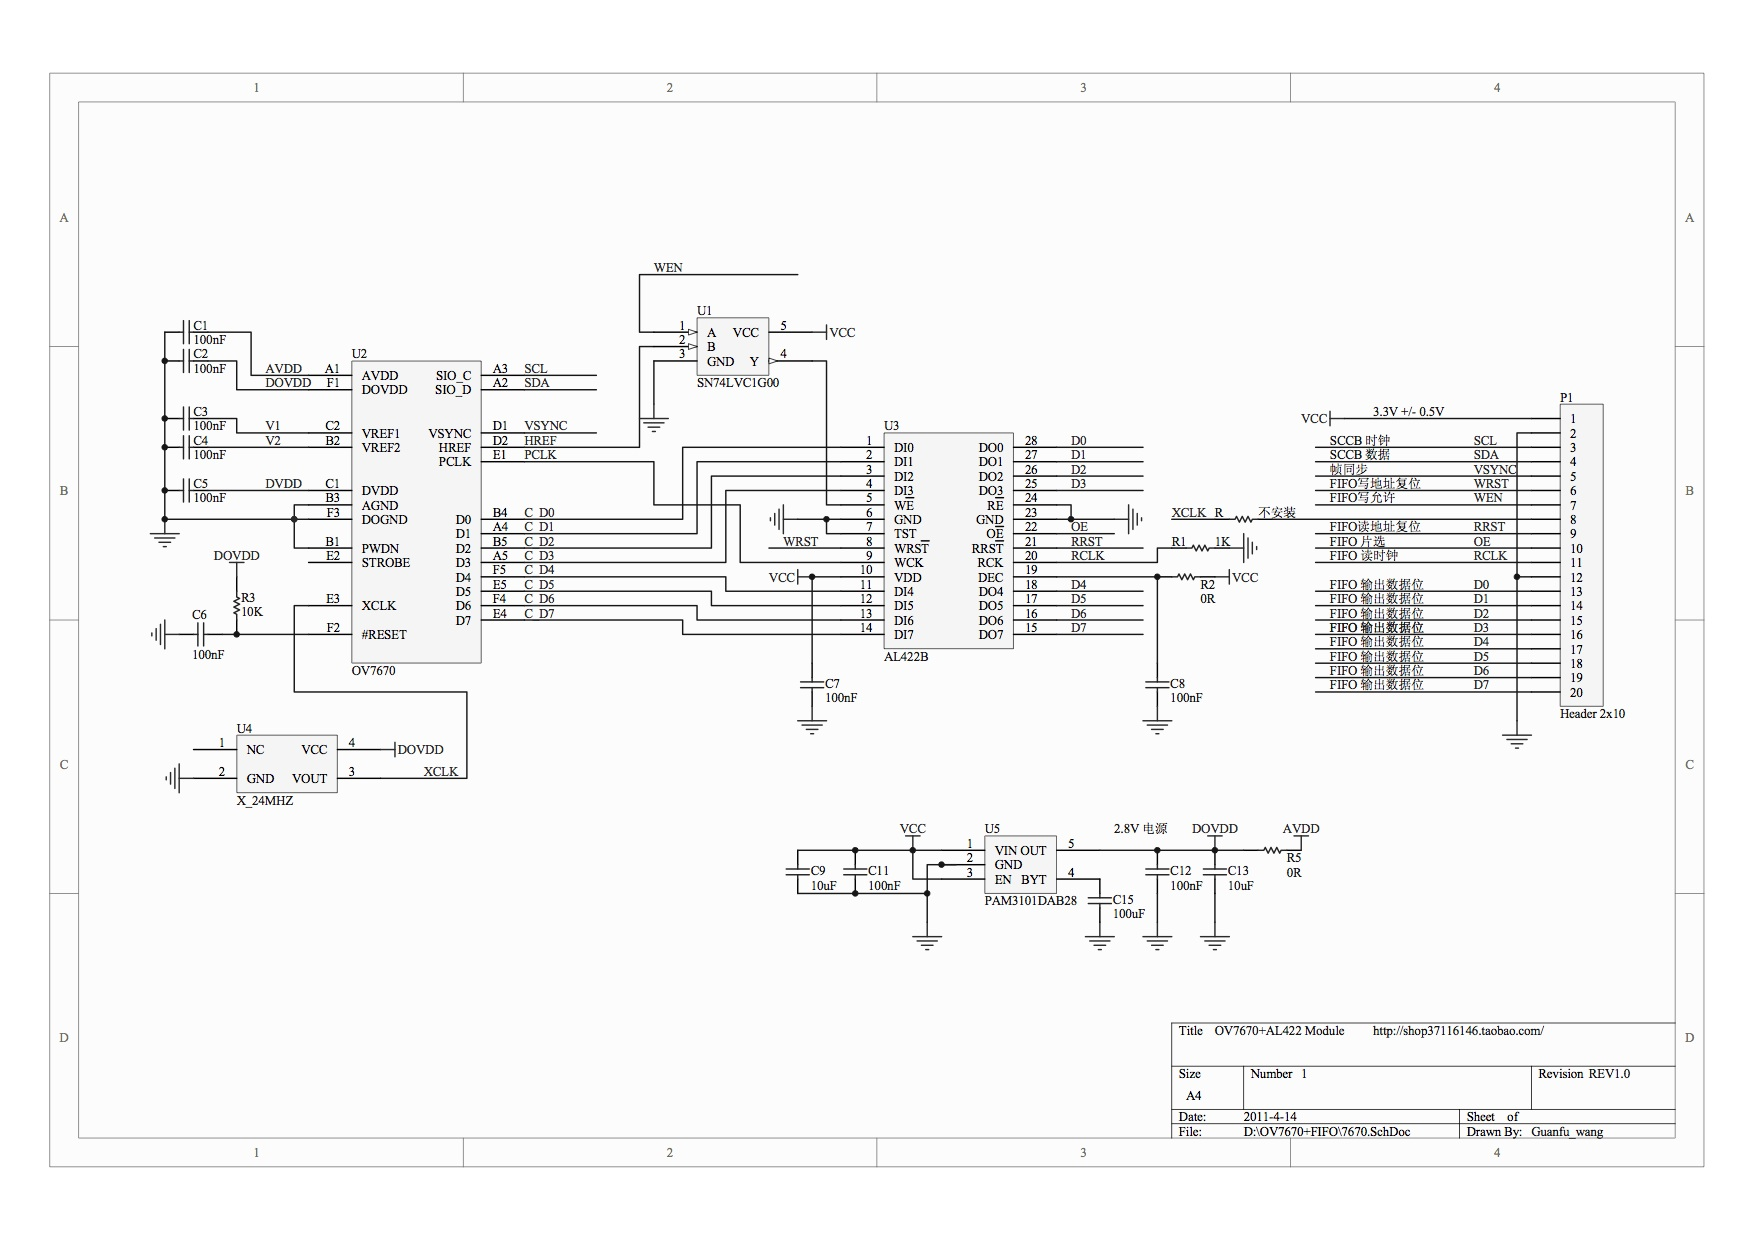
\includegraphics[angle=90,width=\textwidth,height=\textheight-10cm,keepaspectratio]{Figures/OV7670_Schematic.jpg} 
\caption{The circuit diagram for the OV7670 breakout board}
\label{OV7670_Schematic}

\end{figure}
\clearpage
\section{Il Matto and Dual Camera Schematic}\label{sch:IlMatto:Cameras}
\begin{figure}[ht!]
\centering
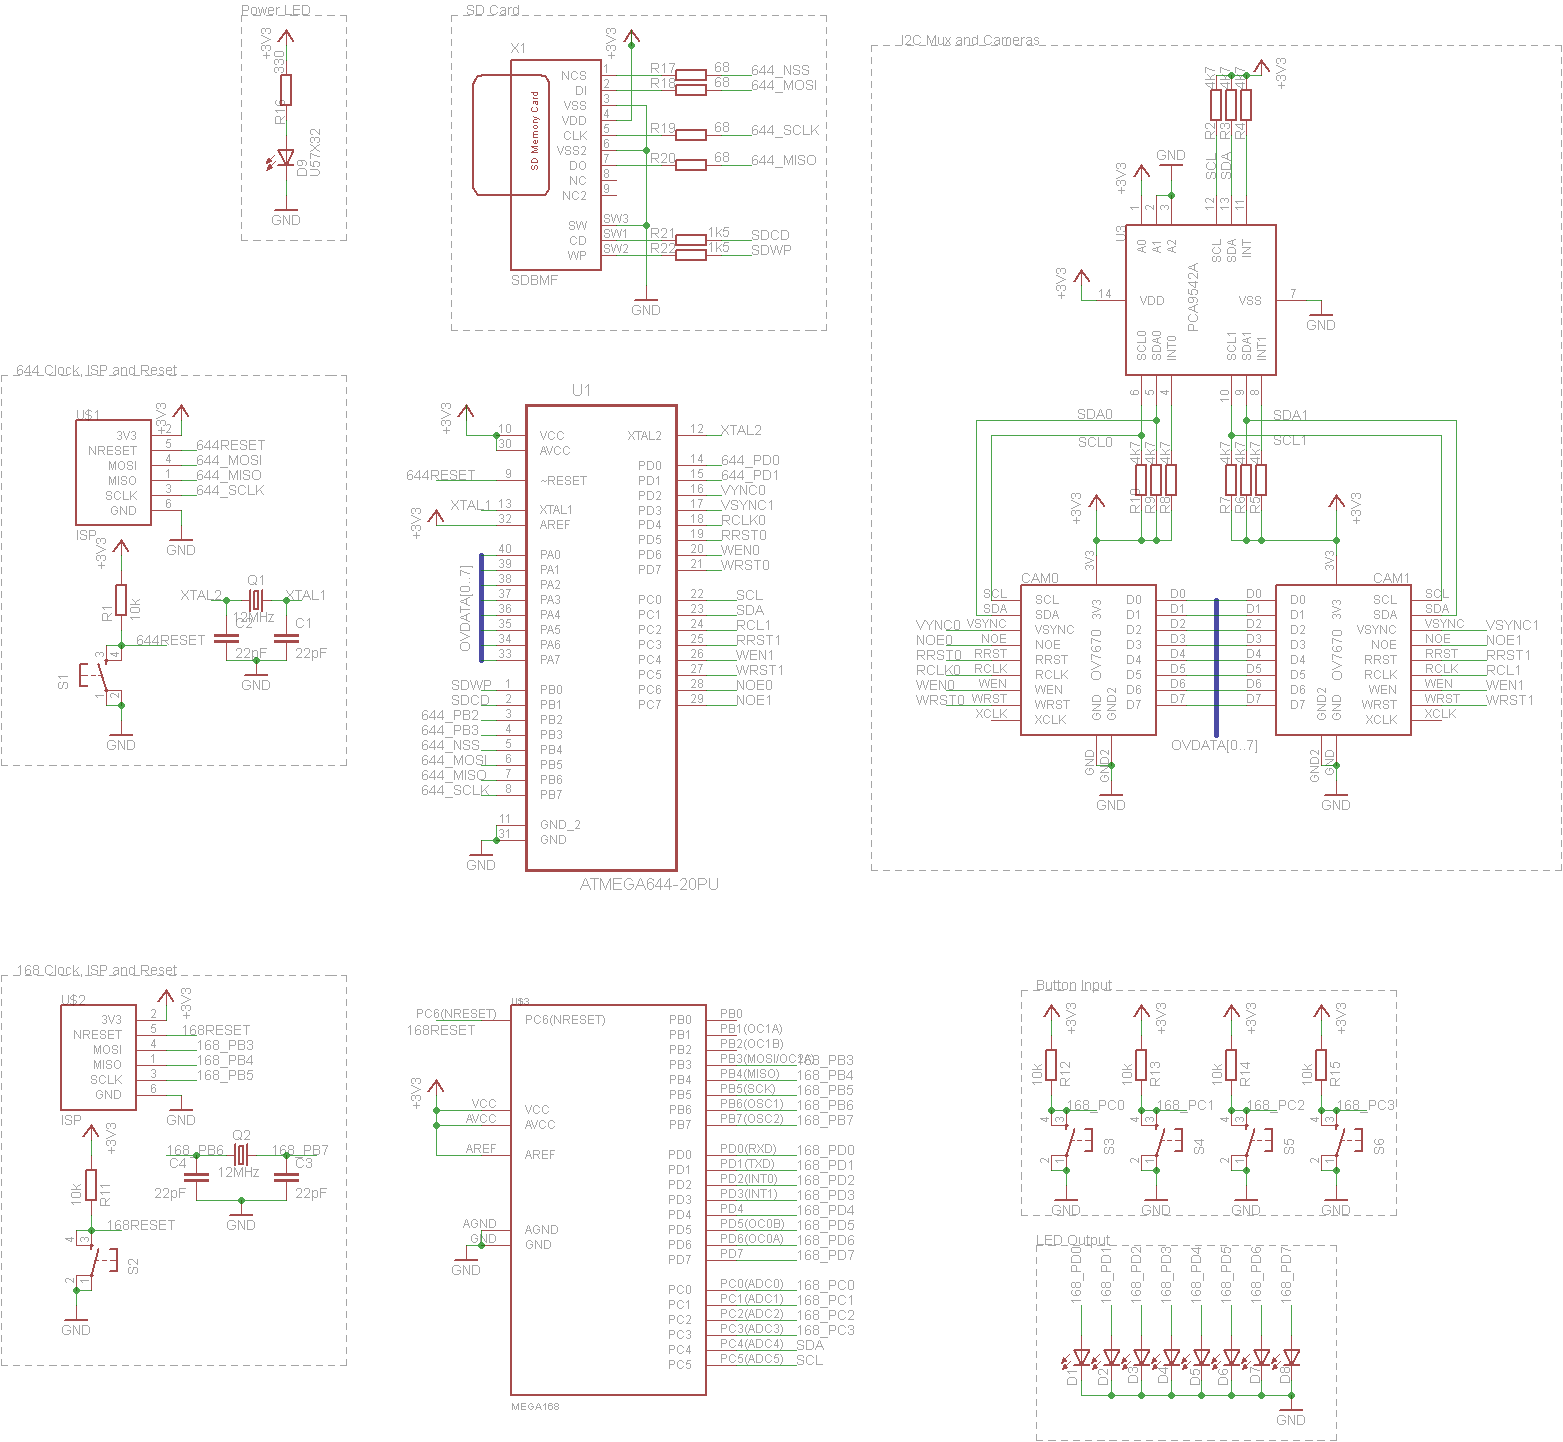
\includegraphics[angle = 90, width=\textwidth,height=\textheight,keepaspectratio]{Figures/IlMattoCamera_CircuitDiagram.png} 
\caption{The circuit diagram for dual cameras using the \textit{Il Matto}}
\label{sch:DualCam_Schematic}
\end{figure}
\clearpage

\section{The Columbus Circuit Diagram} \label{sch:Columbus:CircuitDiagram}
\begin{figure}[ht!]
\centering
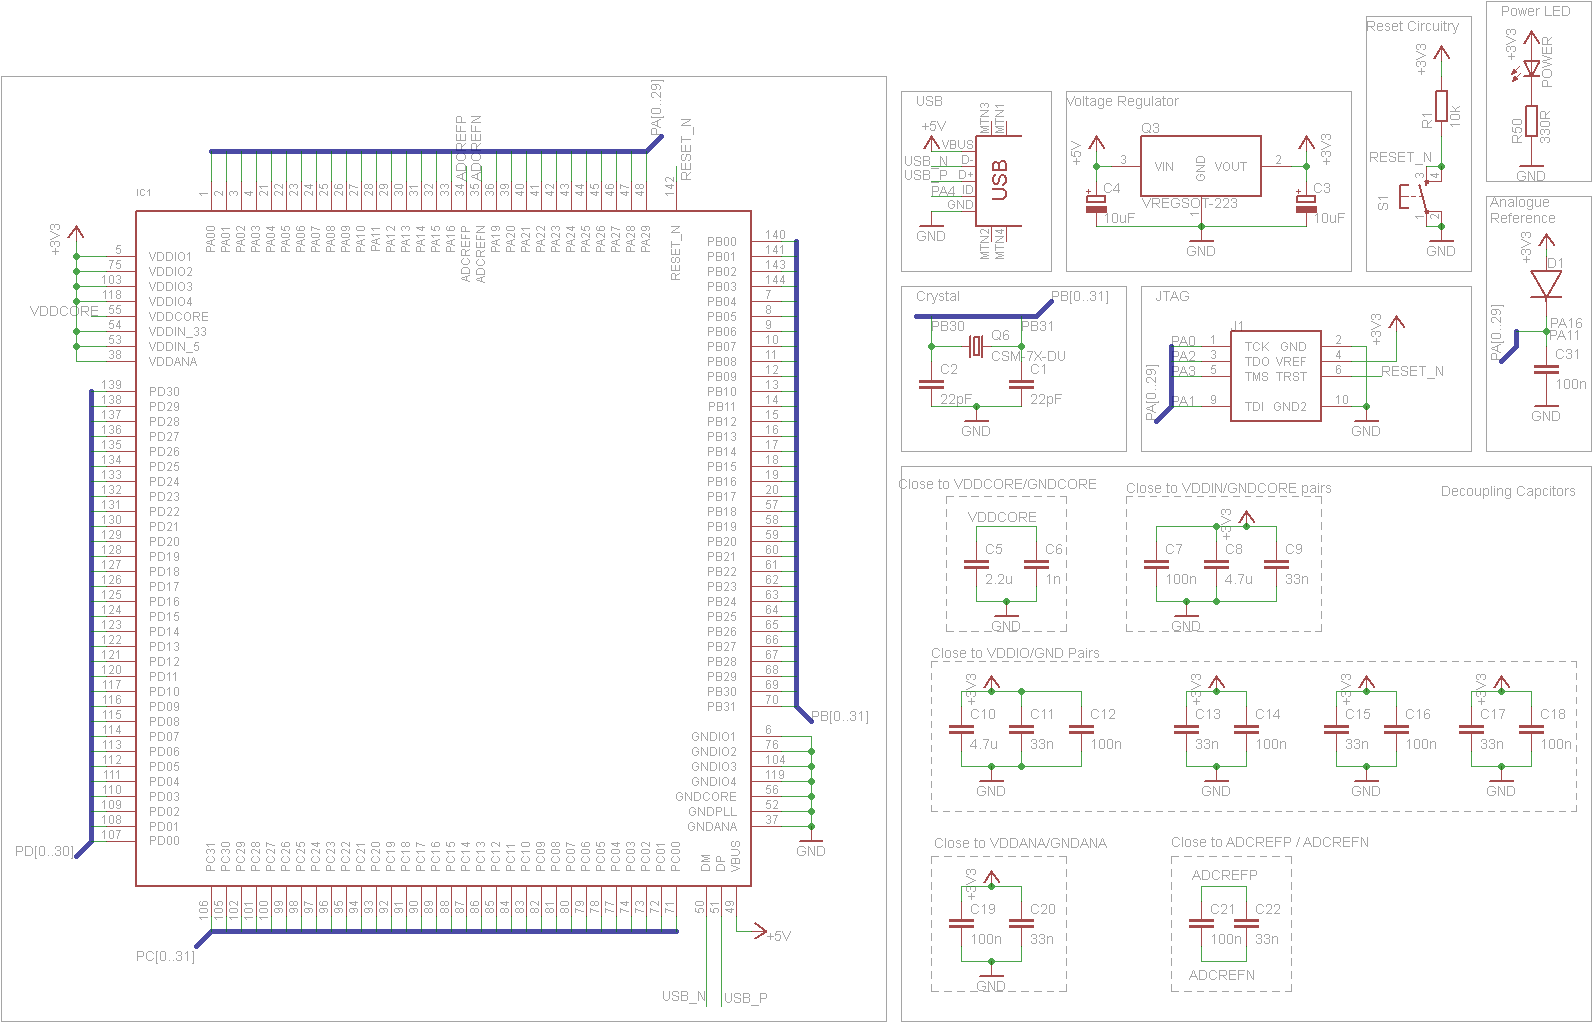
\includegraphics[angle = 90, width=\textwidth,height=\textheight,keepaspectratio]{./Figures/ColumbusCircuitPage1.png}
\caption{The Columbus circuit diagram page 1}
\label{sch:Columbus_Schematic:1}
\end{figure}

\begin{figure}[ht!]
\centering
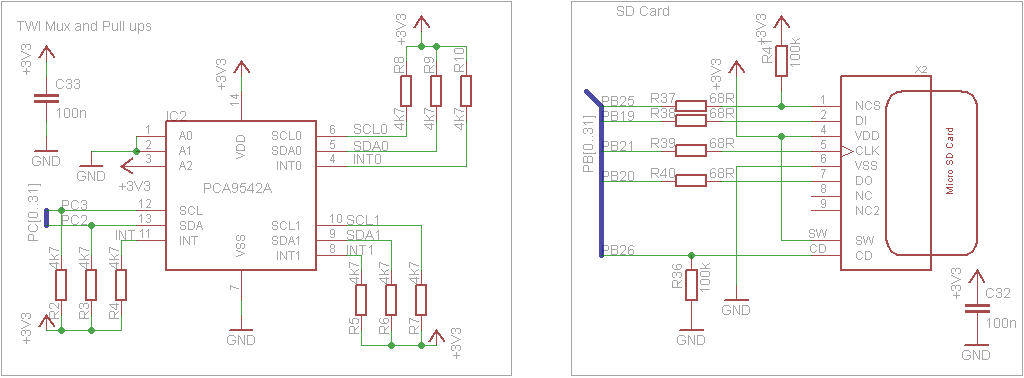
\includegraphics[angle = 90, width=\textwidth,height=\textheight,keepaspectratio]{./Figures/ColumbusCircuitPage2.png}
\caption{The Columbus circuit diagram page 2}
\label{sch:Columbus_Schematic:2}
\end{figure}

\begin{figure}[ht!]
\centering
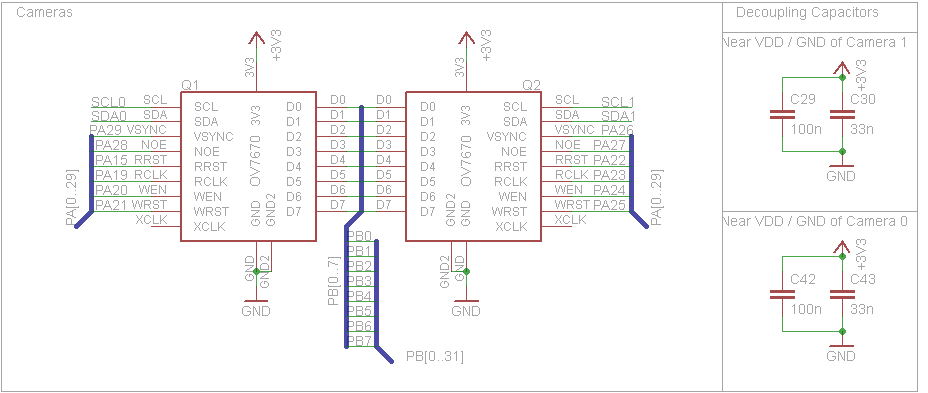
\includegraphics[angle = 90, width=\textwidth,height=\textheight,keepaspectratio]{./Figures/ColumbusCircuitPage3.png}
\caption{The Columbus circuit diagram page 3}
\label{sch:Columbus_Schematic:3}
\end{figure}

\begin{figure}[ht!]
\centering
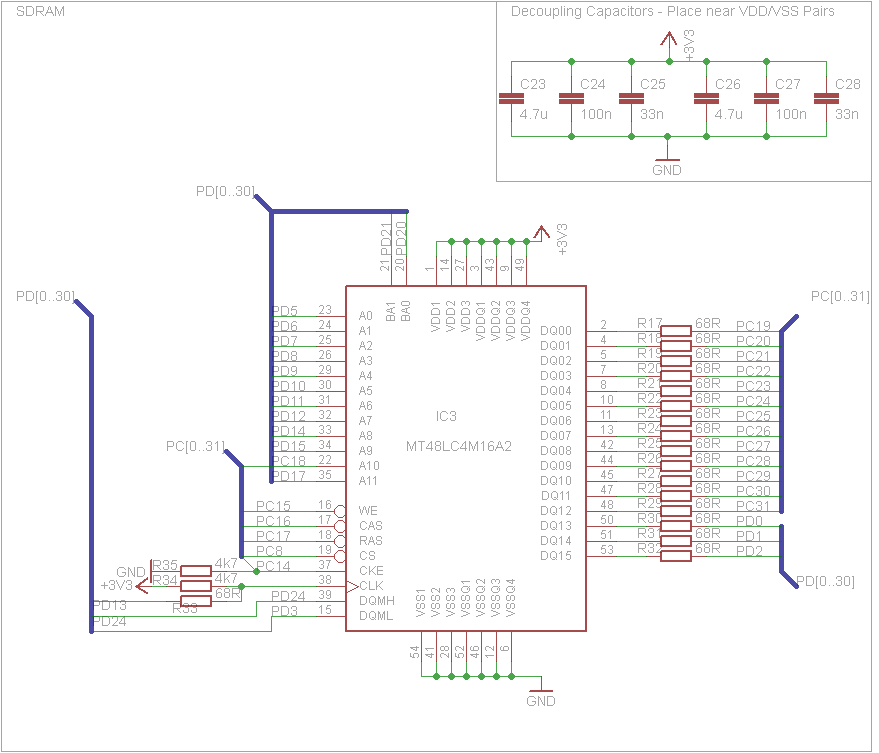
\includegraphics[angle = 90, width=\textwidth,height=\textheight,keepaspectratio]{./Figures/ColumbusCircuitPage4.png}
\caption{The Columbus circuit diagram page 4}
\label{sch:Columbus_Schematic:4}
\end{figure}

\begin{figure}[ht!]
\centering
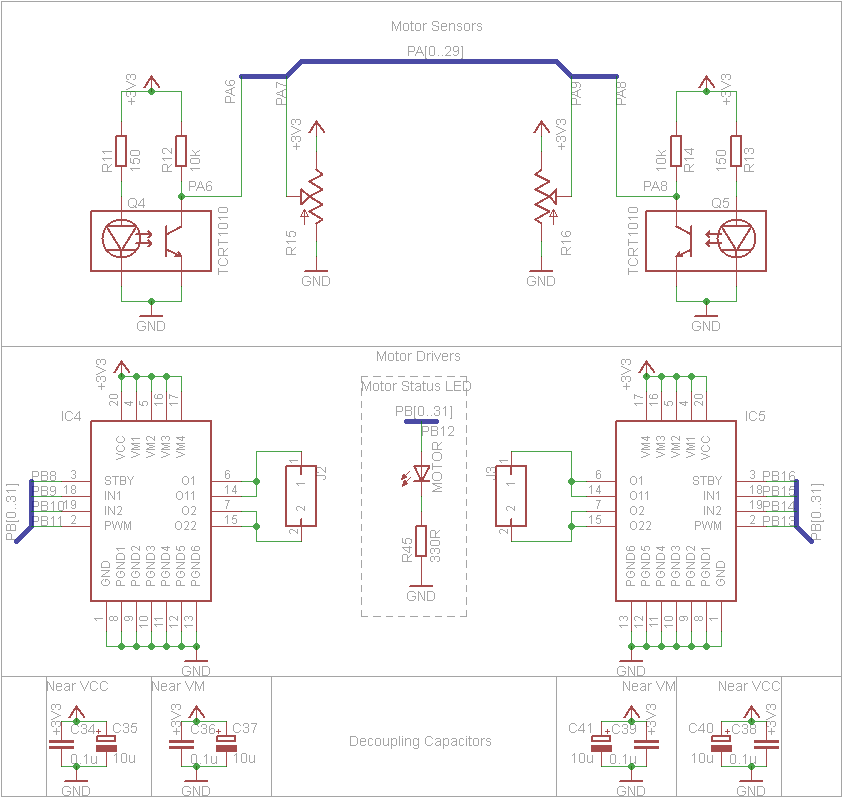
\includegraphics[angle = 90, width=\textwidth,height=\textheight,keepaspectratio]{./Figures/ColumbusCircuitPage5.png}
\caption{The Columbus circuit diagram page 5}
\label{sch:Columbus_Schematic:5}
\end{figure}

\begin{figure}[ht!]
\centering
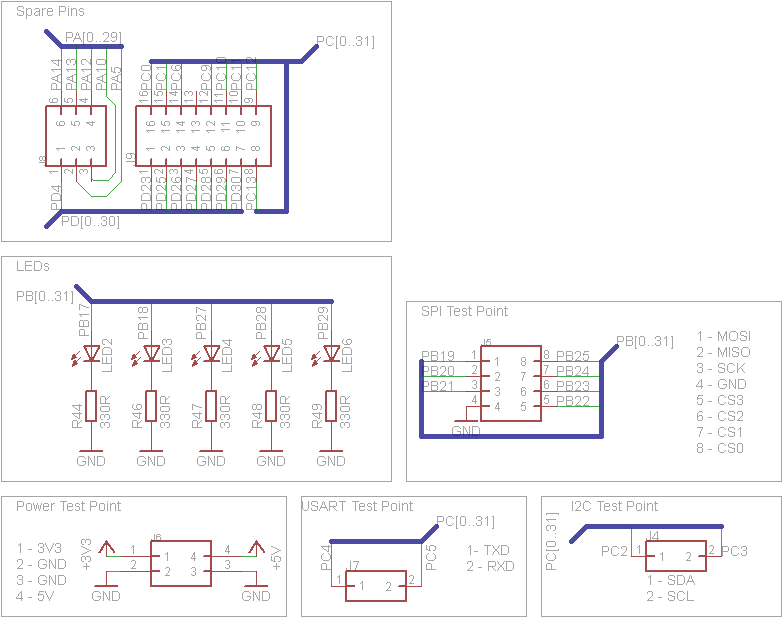
\includegraphics[angle = 90, width=\textwidth,height=\textheight,keepaspectratio]{./Figures/ColumbusCircuitPage6.png}
\caption{The Columbus circuit diagram page 6}
\label{sch:Columbus_Schematic:6}
\end{figure}

